% Options for packages loaded elsewhere
\PassOptionsToPackage{unicode}{hyperref}
\PassOptionsToPackage{hyphens}{url}
%
\documentclass[
  landscape, table]{article}
\usepackage{amsmath,amssymb}
\usepackage{iftex}
\ifPDFTeX
  \usepackage[T1]{fontenc}
  \usepackage[utf8]{inputenc}
  \usepackage{textcomp} % provide euro and other symbols
\else % if luatex or xetex
  \usepackage{unicode-math} % this also loads fontspec
  \defaultfontfeatures{Scale=MatchLowercase}
  \defaultfontfeatures[\rmfamily]{Ligatures=TeX,Scale=1}
\fi
\usepackage{lmodern}
\ifPDFTeX\else
  % xetex/luatex font selection
\fi
% Use upquote if available, for straight quotes in verbatim environments
\IfFileExists{upquote.sty}{\usepackage{upquote}}{}
\IfFileExists{microtype.sty}{% use microtype if available
  \usepackage[]{microtype}
  \UseMicrotypeSet[protrusion]{basicmath} % disable protrusion for tt fonts
}{}
\makeatletter
\@ifundefined{KOMAClassName}{% if non-KOMA class
  \IfFileExists{parskip.sty}{%
    \usepackage{parskip}
  }{% else
    \setlength{\parindent}{0pt}
    \setlength{\parskip}{6pt plus 2pt minus 1pt}}
}{% if KOMA class
  \KOMAoptions{parskip=half}}
\makeatother
\usepackage{xcolor}
\usepackage[margin=1in]{geometry}
\usepackage{graphicx}
\makeatletter
\def\maxwidth{\ifdim\Gin@nat@width>\linewidth\linewidth\else\Gin@nat@width\fi}
\def\maxheight{\ifdim\Gin@nat@height>\textheight\textheight\else\Gin@nat@height\fi}
\makeatother
% Scale images if necessary, so that they will not overflow the page
% margins by default, and it is still possible to overwrite the defaults
% using explicit options in \includegraphics[width, height, ...]{}
\setkeys{Gin}{width=\maxwidth,height=\maxheight,keepaspectratio}
% Set default figure placement to htbp
\makeatletter
\def\fps@figure{htbp}
\makeatother
\setlength{\emergencystretch}{3em} % prevent overfull lines
\providecommand{\tightlist}{%
  \setlength{\itemsep}{0pt}\setlength{\parskip}{0pt}}
\setcounter{secnumdepth}{-\maxdimen} % remove section numbering
\usepackage{amsmath,amssymb}
\usepackage{lmodern}
\usepackage{iftex}
\usepackage[T1]{fontenc}
\usepackage[utf8]{inputenc}
\usepackage{textcomp}
\usepackage[]{microtype}
\usepackage{parskip}
\usepackage[margin=1in]{geometry}
\usepackage{graphicx}
\usepackage{array}
\usepackage{caption,tabularx,booktabs}
\usepackage[default]{opensans}
\usepackage{titling}
\usepackage{microtype}
\usepackage{letterspace}
\setlength{\droptitle}{-4em}
\ifLuaTeX
  \usepackage{selnolig}  % disable illegal ligatures
\fi
\IfFileExists{bookmark.sty}{\usepackage{bookmark}}{\usepackage{hyperref}}
\IfFileExists{xurl.sty}{\usepackage{xurl}}{} % add URL line breaks if available
\urlstyle{same}
\hypersetup{
  pdftitle={Alaska Primary Care Association},
  hidelinks,
  pdfcreator={LaTeX via pandoc}}

\title{Alaska Primary Care Association}
\author{}
\date{\vspace{-2.5em}}

\begin{document}
\maketitle

\definecolor{lightgreen}{RGB}{144,238,144}
\definecolor{yellow}{RGB}{255,255,0}
\definecolor{lightpink}{RGB}{255,192,203}

\begin{table}[!h]
\centering
\fontsize{8}{10}\selectfont
\begin{tabular}[t]{>{\raggedright\arraybackslash}m{1in}|r|r|r|r|r|r|r|>{\raggedleft\arraybackslash}m{0.5in}|>{\raggedleft\arraybackslash}m{0.5in}|r|>{\raggedleft\arraybackslash}m{0.5in}|>{\raggedright\arraybackslash}m{0.5in}|>{\raggedleft\arraybackslash}m{0.5in}|>{\raggedright\arraybackslash}m{0.5in}}
\hline
Performance Metric & 12.31.2021 & 03.31.2022 & 06.30.2022 & 09.30.2022 & 12.31.2022 & 03.31.2023 & 06.30.2023 & 03.31.2022
Y1 Target & 03.31.2023
Y2 Target & 03.31.2024
Y3 Target & Cumulative Target & \% of Cumulative Target & Total Target & \% of Total Target\\
\hline
Total Participants Served & 145 & 145 & 244 & 244 & 114 & 114 & 137 & 100 & 115 & 115 & 330 & \cellcolor{lightgreen}{42\%} & 440 & 31\%\\
\hline
Participants Began Ed/Job Training & 145 & 145 & 244 & 244 & 114 & 114 & 137 & 100 & 115 & 115 & 330 & \cellcolor{lightgreen}{42\%} & 440 & 31\%\\
\hline
Participants Completed Training & 8 & 13 & 37 & 37 & 25 & 53 & 68 & 6 & 70 & 92 & 168 & \cellcolor{lightgreen}{40\%} & 341 & 20\%\\
\hline
Total Participants Completed and Obtained Credential & 8 & 13 & 37 & 37 & 25 & 30 & 20 & 6 & 70 & 92 & 168 & \cellcolor{yellow}{12\%} & 341 & 6\%\\
\hline
Entered Employment & 3 & 3 & 3 & 3 & 0 & 0 & 0 & 0 & 35 & 39 & 74 & \cellcolor{yellow}{0\%} & 140 & 0\%\\
\hline
Incumbent Workers Advanced & 0 & 0 & 23 & 23 & 16 & 0 & 0 & 3 & 18 & 30 & 51 & \cellcolor{yellow}{0\%} & 81 & 0\%\\
\hline
\end{tabular}
\end{table}

*\% of Current Year Target calculated as most recently available
quarterly data divided by sum of cumulative milestones-to-date.
e.g.~Year 2 milestone is sum of Year 1 \& Year 2 annual milestones.

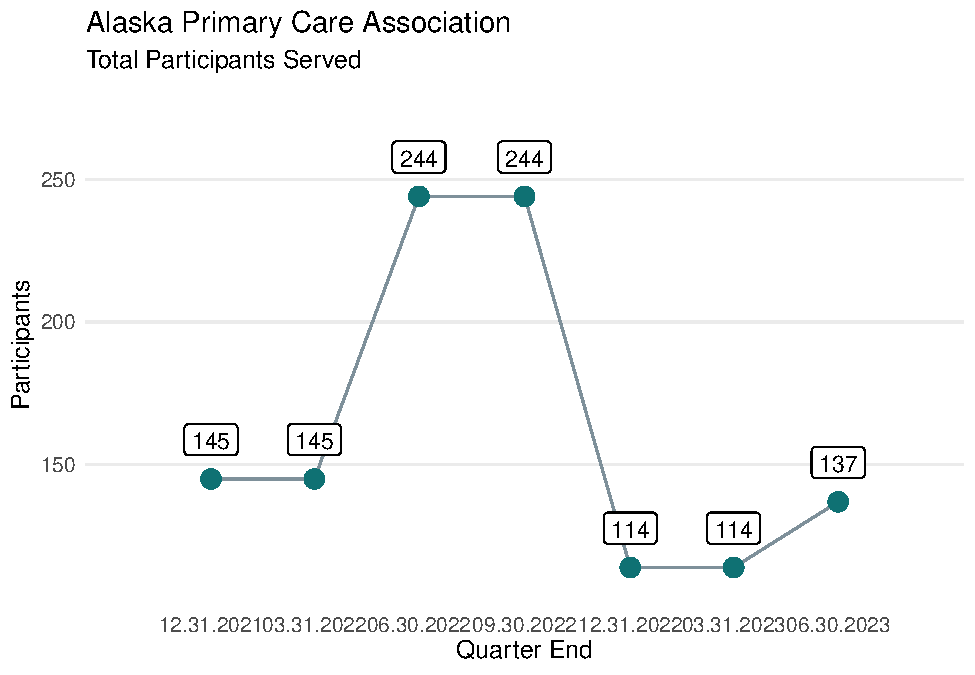
\includegraphics{rh_pdf_by_grantee_files/figure-latex/unnamed-chunk-4-1.pdf}

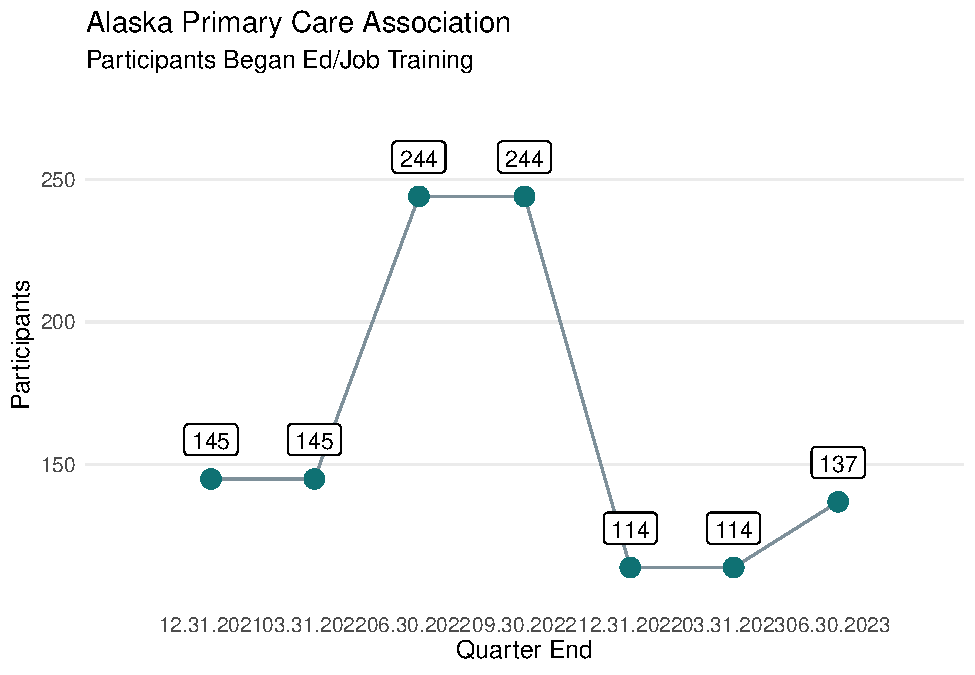
\includegraphics{rh_pdf_by_grantee_files/figure-latex/unnamed-chunk-5-1.pdf}

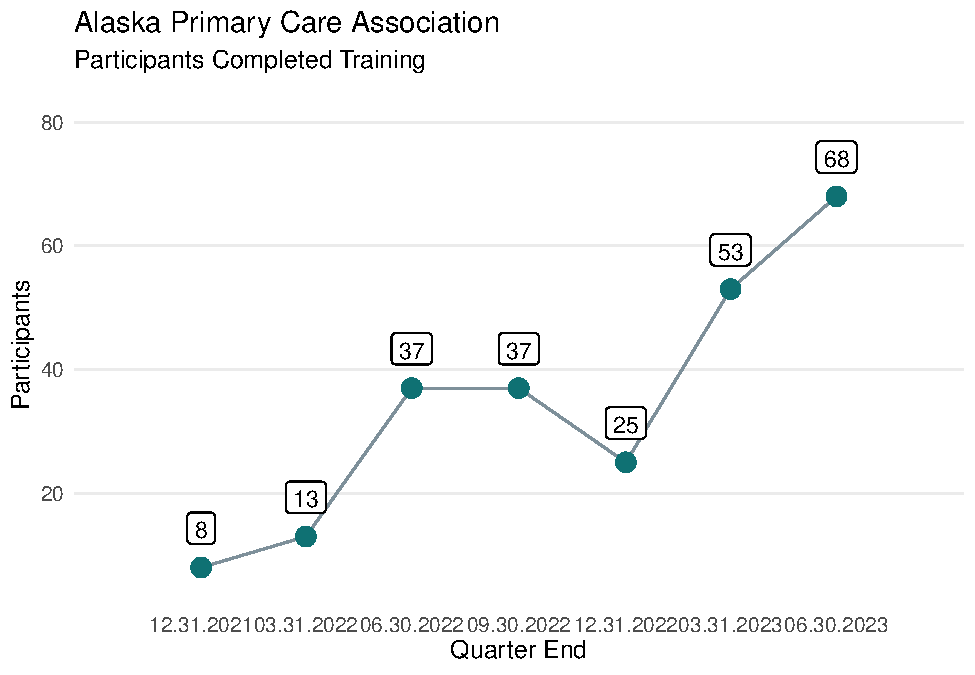
\includegraphics{rh_pdf_by_grantee_files/figure-latex/unnamed-chunk-6-1.pdf}

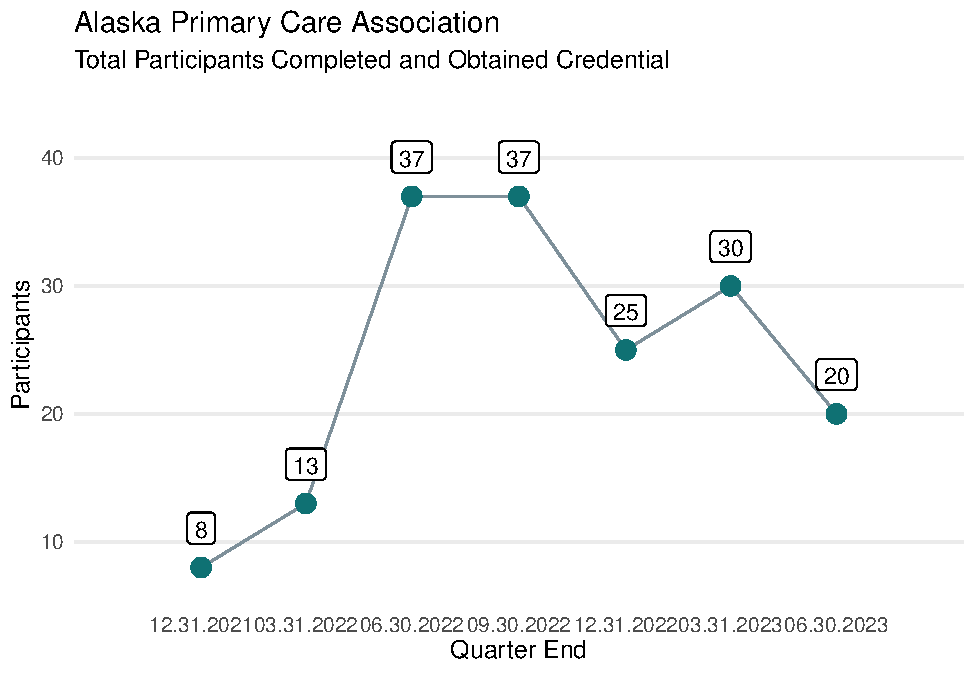
\includegraphics{rh_pdf_by_grantee_files/figure-latex/unnamed-chunk-7-1.pdf}

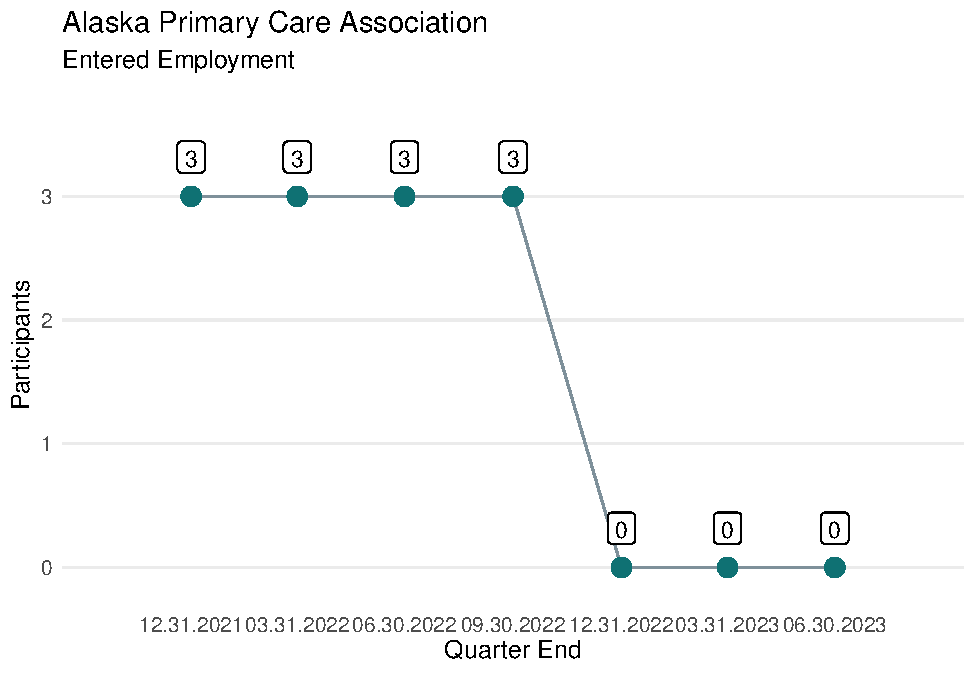
\includegraphics{rh_pdf_by_grantee_files/figure-latex/unnamed-chunk-8-1.pdf}

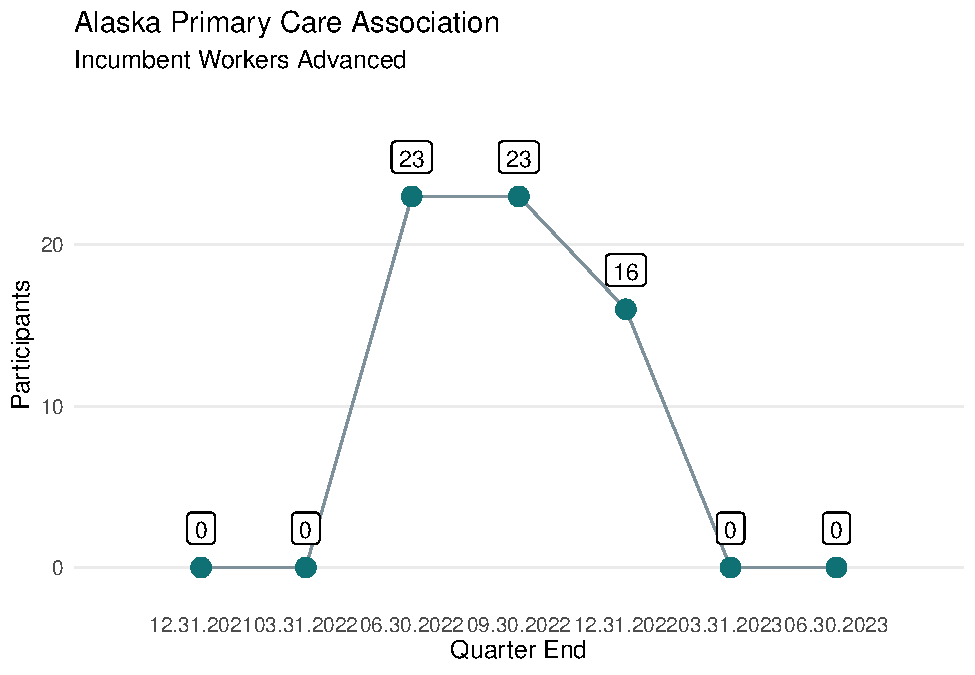
\includegraphics{rh_pdf_by_grantee_files/figure-latex/unnamed-chunk-9-1.pdf}

\end{document}
